%input macros (i.e. write your own macros file called MacroFile1.tex)
    %\newcommand{\PdfPsText}[2]{
  \ifpdf
     #1
  \else
     #2
  \fi
}

\newcommand{\IncludeGraphicsH}[3]{
  \PdfPsText{\includegraphics[height=#2]{#1}}{\includegraphics[bb = #3, height=#2]{#1}}
}

\newcommand{\IncludeGraphicsW}[3]{
  \PdfPsText{\includegraphics[width=#2]{#1}}{\includegraphics[bb = #3, width=#2]{#1}}
}

\newcommand{\InsertFig}[3]{
  \begin{figure}[!htbp]
    \begin{center}
      \leavevmode
      #1
      \caption{#2}
      \label{#3}
    \end{center}
  \end{figure}
}


%%% Local Variables: 
%%% mode: latex
%%% TeX-master: "~/Documents/LaTeX/CUEDThesisPSnPDF/thesis"
%%% End: 



\documentclass[oneside,12pt]{CUEDthesisPSnPDF}
\begin{document}

\renewcommand{\thepage}{\mbox{A-\arabic{page}}}
\renewcommand\thechapter{\Alph{chapter}}
\renewcommand{\chaptername}{Appendix}
\renewcommand{\thefigure}{A-\arabic{chapter}.\arabic{figure}}
\renewcommand{\thetable}{A-\arabic{chapter}.\arabic{table}}
\setcounter{page}{21}
\addtocounter{chapter}{1}

\chapter{Process model of leaky bucket}
\thispagestyle{fancy}
\begin{figure}[!htb]
\centering
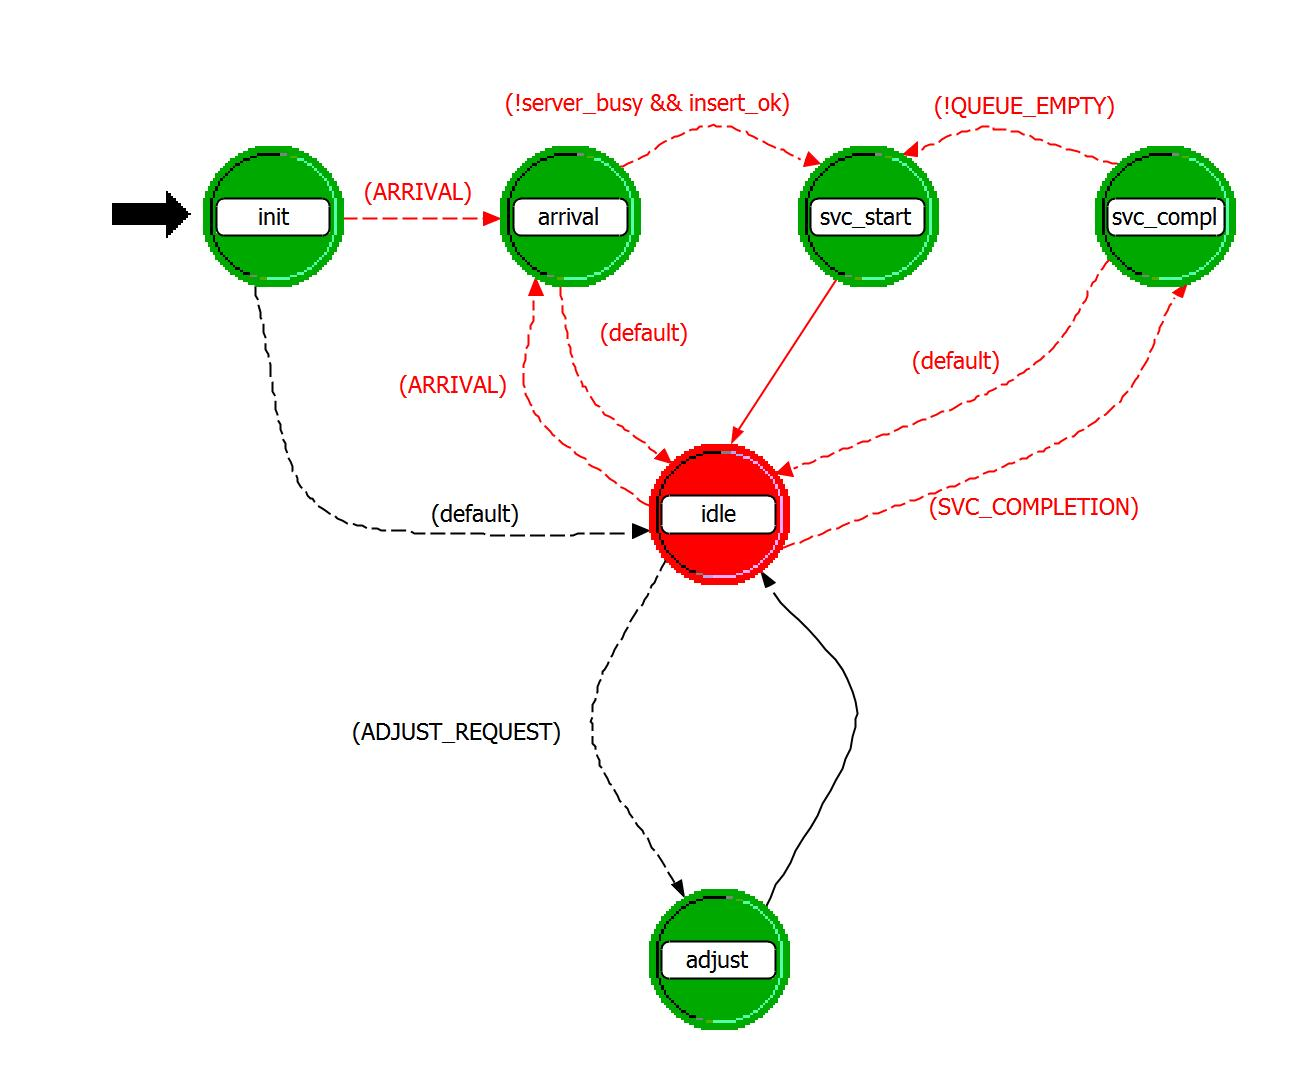
\includegraphics[width=2.6in]{fig/lb}
\caption{process model of leaky bucket}
\label{fig:leaky_bucket}
\end{figure}

Leaky bucket is similar to finite queuing system. So I implement leaky bucket based on \verb|acb-fifo| queue model. Each burst generation queue equip a leaky bucket as traffic shaper or rate controller. The rate-determine algorithm reside in \verb|adjust| state. It is responsible for receiving feedback message from core node and direct to adjust transmission rate. 

\end{document}
